\documentclass[UTF8,fontset=none,12pt]{ctexart}

\setCJKmainfont{Songti SC}
\setCJKsansfont{PingFang SC}
\setCJKmonofont{Songti SC}

\usepackage[a4paper,margin=2.35cm]{geometry}
\usepackage{amsmath,amssymb,amsthm,mathtools,bm}
\usepackage{graphicx}
\usepackage{float}
\usepackage{booktabs}
\usepackage{enumitem}
\usepackage[hidelinks]{hyperref}

\newcommand{\C}{\mathbb{C}}
\newcommand{\R}{\mathbb{R}}
\newcommand{\rank}{\operatorname{rank}}

\title{数值线性代数\quad 第 9 讲：MATLAB 数值实验}
\author{Lloyd N. Trefethen、David Bau III\quad 中文阅读版}
\date{}

\begin{document}
\maketitle
\pagestyle{plain}

要学好数值线性代数，必须养成在计算机上做实验的习惯. MATLAB\textsuperscript{\textregistered} 是进行这类实验的优秀问题求解环境.本讲通过三个例子展示 MATLAB 实验，同时观察 Gram--Schmidt 正交化的稳定性.

\section*{MATLAB}

MATLAB 是一种用于数学计算的语言，基本数据类型是向量和矩阵.它与 Fortran、C 等语言的区别之一，是工作在更高的数学抽象层次上：矩阵求逆、奇异值分解、快速 Fourier 变换等数百种操作都以内置命令提供.它同时也是一个问题求解环境，由解释器处理顶层命令而不是由编译器先编译，并且可以直接访问二维和三维图形功能.

自 20 世纪 80 年代以来，MATLAB 已成为全世界数值分析人员和工程师广泛使用的工具.对于大规模科学计算中的许多问题，以及数值线性代数中几乎所有小型和中型实验，MATLAB 都是首选语言.

本书会不时使用 MATLAB 展示数值实验，也会在习题中使用它.由于实验数量有限，而且读者只需具备阅读 MATLAB 代码的能力就能跟上，本书不系统介绍这门语言.

\paragraph{商标注.} MATLAB 是 The MathWorks, Inc. 的注册商标，地址为 24 Prime Park Way, Natick, MA 01760, USA；原书还列出电话 508-647-7000、传真 508-647-7001、电子邮箱 \texttt{info@mathworks.com} 和网址 \url{http://wsrv.mathworks.com}.

\section*{实验 1：离散 Legendre 多项式}

第 7 讲考察了定义在区间 $[-1,1]$ 上、列由单项式 $1,x,x^2,x^3$ 组成的 Vandermonde “矩阵”.现在把 $[-1,1]$ 离散成 257 个等距点，就得到真正的 Vandermonde 矩阵.下面的 MATLAB 代码构造该矩阵并计算其约化 QR 分解.

\begin{verbatim}
x = (-128:128)'/128;        % Set x to a discretization of [-1,1].
A = [x.^0 x.^1 x.^2 x.^3]; % Construct Vandermonde matrix.
[Q,R] = qr(A,0);            % Find its reduced QR factorization.
\end{verbatim}

逐行看这些命令.第一行的撇号把行向量 $(-128:128)$ 转成列向量.第二行的点号乘方运算符表示逐元素乘方.第三行的 `qr` 是 MATLAB 中计算 QR 分解的内置函数，参数 0 表示需要约化分解而不是完整分解.这里使用的并不是 Gram--Schmidt 正交化，而是下一讲讨论的 Householder 三角化；不过对于当前实验，这一差别不影响目的.三行末尾的分号会抑制原本会打印出的 $x,A,Q,R$.

矩阵 $Q$ 的列与图 7.1 中前四个 Legendre 多项式基本一致.由于定义 Legendre 多项式的 $[-1,1]$ 连续内积被离散内积替代，两者会有接近绘图精度的细微差异；此外归一化方式也不同，因为 Legendre 多项式应满足 $P_k(1)=1$.可以把 $Q$ 的每一列除以该列最后一个元素来修正这一点：

\begin{verbatim}
scale = Q(257,:);              % Select last row of Q.
Q = Q*diag(1 ./scale);         % Rescale columns by these numbers.
plot(Q)                        % Plot columns of rescaled Q.
\end{verbatim}

计算结果是一幅与图 7.1 很相似的图（原书没有重复展示）.如果用 Fortran 或 C 完成同样的工作，通常需要几十行代码，其中包含许多循环和嵌套循环.而在这里的六行 MATLAB 代码中，没有一个循环显式出现，尽管每一行至少隐含了一个循环.

\section*{实验 2：经典 Gram--Schmidt 与修改后的 Gram--Schmidt}

第二个例子包含更多算法内容，目的是探索经典 Gram--Schmidt 与修改后的 Gram--Schmidt 在数值稳定性上的差异.

首先构造一个方阵 $A$，其左右奇异向量随机生成，奇异值从 $2^{-1}$ 到 $2^{-80}$，相邻奇异值相差一个因子 2：

\begin{verbatim}
[U,X] = qr(randn(80));       % Set U to a random orthogonal matrix.
[V,X] = qr(randn(80));       % Set V to a random orthogonal matrix.
S = diag(2.^(-1:-1:-80));    % Set S to exponentially graded entries.
A = U*S*V;                   % Set A to have these singular values.
\end{verbatim}

这里的实正交矩阵 $U,V$ 使 $A$ 具有所需的奇异值；右侧矩阵写成 $V$ 或等价地重新命名右奇异向量都不影响这个实验的目的.

接下来用算法 7.1 和算法 8.1 计算 $A$ 的 QR 分解.其中 `clgs` 和 `mgs` 是分别实现这两个算法的 MATLAB 程序，本讲不列出其完整代码：

\begin{verbatim}
[QC,RC] = clgs(A);           % Classical Gram--Schmidt.
[QM,RM] = mgs(A);            % Modified Gram--Schmidt.
\end{verbatim}

最后比较两次计算得到的对角元 $r_{jj}$（MATLAB 绘图代码略）.由于
\[
    r_{jj}=\|P_ja_j\|_2,
\]
这些数描绘了每一步投影的大小.结果用对数坐标画在图 9.1 中.

首先可以看到，$r_{jj}$ 随 $j$ 稳定下降，和直线 $2^{-j}$ 很接近.当然，$r_{jj}$ 并不严格等于 $A$ 的第 $j$ 个奇异值，但它是一个相当好的近似.对此可以做如下粗略解释.按式 (5.3)，$A$ 的 SVD 可以写成
\[
    A=2^{-1}u_1v_1^*+2^{-2}u_2v_2^*+2^{-3}u_3v_3^*+\cdots+2^{-80}u_{80}v_{80}^*,
\]
其中 $\{u_j\}$ 与 $\{v_j\}$ 分别是 $A$ 的左右奇异向量.因此，$A$ 的第 $j$ 列形如
\[
    a_j=2^{-1}\overline{v_{j1}}u_1+2^{-2}\overline{v_{j2}}u_2+2^{-3}\overline{v_{j3}}u_3+\cdots+2^{-80}\overline{v_{j,80}}u_{80}.
\]
由于奇异向量是随机的，可以预计这些数 $v_{ji}$ 的量级大致相同，约为 $80^{-1/2}\approx0.1$.做 QR 分解时，第一个向量 $q_1$ 很可能近似 $u_1$，而 $r_{11}$ 的量级约为 $2^{-1}\times80^{-1/2}$.下一步正交化得到的 $q_2$ 很可能近似 $u_2$，$r_{22}$ 的量级约为 $2^{-2}\times80^{-1/2}$，依此类推.

图 9.1 的第二个现象是，$r_{jj}$ 的几何下降不会一直持续到 $j=80$.这是计算机舍入误差的结果.对于经典 Gram--Schmidt，数值不会低于约 $10^{-8}$；对于修改后的 Gram--Schmidt，它们还会继续下降约 8 个数量级，达到 $10^{-16}$ 的量级，也就是本次计算所用计算机的机器 epsilon 水平.机器 epsilon 将在第 13 讲定义.

显然，不同算法的稳定性可能不同.经典 Gram--Schmidt 已被充分证明属于不稳定算法，因此很少使用；有时它会在并行计算机上出现，因为通信方面的优势可能抵消其不稳定性的缺点.

\begin{figure}[H]
    \centering
    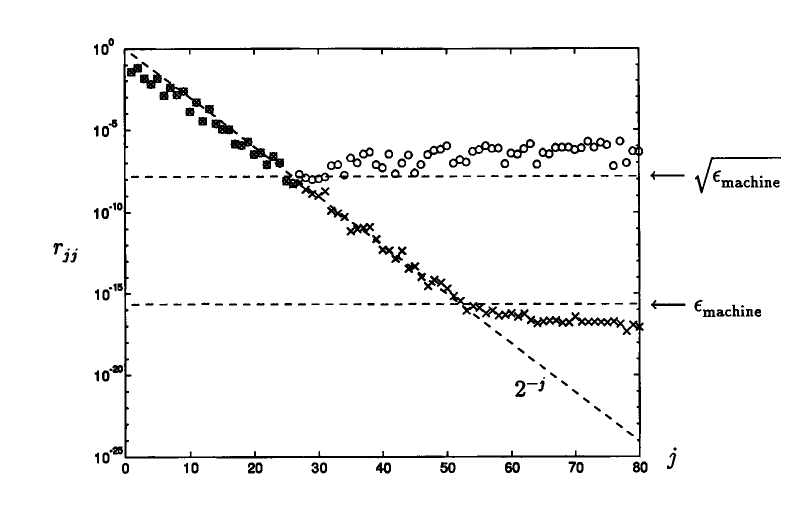
\includegraphics[width=0.80\linewidth]{../assets/figure-9-1.png}
    \caption{指数分级奇异值矩阵的 QR 分解中计算得到的 $r_{jj}$ 与 $j$ 的关系.圆圈表示经典 Gram--Schmidt，叉号表示修改后的 Gram--Schmidt；虚线标出了 $2^{-j}$、$\sqrt{\epsilon_{\mathrm{machine}}}$ 和 $\epsilon_{\mathrm{machine}}$ 等尺度.}
    \label{fig:9-1}
\end{figure}

\section*{实验 3：正交性的数值丢失}

连续介绍两个不稳定现象可能会让读者有些混乱，但本讲最后再展示一种不同的现象：经典和修改后的 Gram--Schmidt 都可能产生彼此远非正交的向量 $q_i$.当 $A$ 接近秩亏时，正交性会丢失；和许多数值不稳定性一样，它甚至可以在很低的维数中出现.

先在纸上考虑矩阵
\begin{equation}
    A=\begin{bmatrix}
        0.70000&0.70711\\
        0.70001&0.70711
    \end{bmatrix}.
    \tag{9.1}
\end{equation}
假设计算机把所有计算结果舍入到五位有效数字（第 13 讲将讨论浮点运算）.在 $2\times2$ 情形中，经典与修改后的算法相同.第 $j=1$ 步归一化第一列，得到
\[
    r_{11}=0.98996,\qquad
    q_1=a_1/r_{11}
    =\begin{bmatrix}0.70000/0.98996\\0.70001/0.98996\end{bmatrix}
    =\begin{bmatrix}0.70710\\0.70711\end{bmatrix}
\]
（均按五位有效数字计算）.第 $j=2$ 步计算并减去 $a_2$ 在 $q_1$ 方向上的分量：
\[
    r_{12}=q_1^*a_2
    =0.70710\times0.70711+0.70711\times0.70711=1.0000,
\]
\[
    v_2=a_2-r_{12}q_1
    =\begin{bmatrix}0.70711\\0.70711\end{bmatrix}
     -\begin{bmatrix}0.70710\\0.70711\end{bmatrix}
    =\begin{bmatrix}0.00001\\0.00000\end{bmatrix}.
\]
这个计算得到的 $v_2$ 几乎完全由误差支配.最终得到的 $Q$ 为
\[
    Q=\begin{bmatrix}0.70710&1.0000\\0.70711&0.0000\end{bmatrix},
\]
它与任何正交矩阵都不接近.

即使使用十六位有效数字，把修改后的 Gram--Schmidt 用在式 (9.1) 上仍会损失大约 5 位正交性.下面给出 MATLAB 证据；`eye` 函数生成指定维数的单位矩阵：

\begin{verbatim}
A = [.70000 .70711       % Define A.
     .70001 .70711];
[Q,R] = qr(A);            % Compute factor Q by Householder.
norm(Q'*Q-eye(2))        % Test orthogonality of Q.
[Q,R] = mgs(A);           % Compute factor Q by modified G-S.
norm(Q'*Q-eye(2))        % Test orthogonality of Q.
\end{verbatim}

不带分号的行会打印
\[
    \texttt{ans = 2.3515e-16},\qquad
    \texttt{ans = 2.3014e-11}.
\]

\section*{习题}

\begin{enumerate}[label=\textbf{9.\arabic*}]
    \item
    \begin{enumerate}[label=(\alph*)]
        \item 运行实验 1 的六行 MATLAB 程序，生成近似的 Legendre 多项式图.
        \item 对 $k=0,1,2,3$，在 257 点网格上画出这些近似多项式与精确多项式 (7.11) 的差.误差有多大？如何分布？
        \item 将这些结果与网格间距 $\Delta x=2^{-\nu}$、不同 $\nu$ 的结果比较.看起来是哪一个 $\Delta x$ 的幂控制收敛速度？
    \end{enumerate}

    \item 在实验 2 中，$A$ 的奇异值与 QR 因子 $R$ 的对角元近似相等.现在考虑一个很不同的例子.设 $Q=I$、$A=R$，其中 $A$ 是 $m\times m$ Toeplitz 矩阵：主对角线全为 1，第一条上对角线全为 2，其余元素为 0.
    \begin{enumerate}[label=(\alph*)]
        \item $A$ 的特征值、行列式和秩分别是什么？
        \item $A^{-1}$ 是什么？
        \item 给出 $\sigma_m$（$A$ 的第 $m$ 个奇异值）的一个非平凡上界.可以用 MATLAB 获取直觉，但上界必须给出解析证明.提示：使用 (b).
    \end{enumerate}
    这个问题说明，不能总是从矩阵的特征值或 QR 因子 $R$ 的对角元推断其奇异值的详细信息.

    \item
    \begin{enumerate}[label=(\alph*)]
        \item 编写 MATLAB 程序，建立一个 $15\times40$ 的矩阵，除下图所示位置为 1 外其余元素全为 0.最左上角的 1 位于 $(2,2)$，最右下角的 1 位于 $(13,39)$.该图由命令 `spy(A)` 生成.
    \end{enumerate}

    \begin{figure}[H]
        \centering
        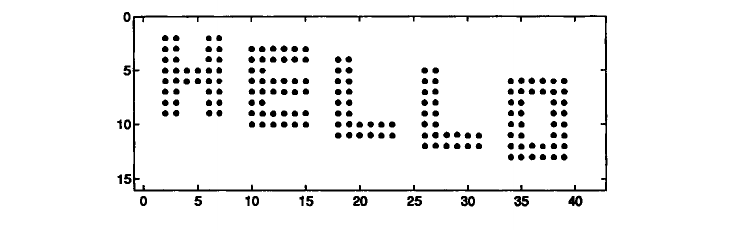
\includegraphics[width=0.78\linewidth]{../assets/figure-9-3-spy.png}
        \caption{习题 9.3 中稀疏矩阵的 `spy(A)` 图.}
        \label{fig:9-3-spy}
    \end{figure}

    \begin{enumerate}[label=(\alph*),start=2]
        \item 调用 `svd` 计算 $A$ 的奇异值并打印结果.同时用 `plot` 和 `semilogy` 画出这些数. $A$ 的数学精确秩是多少？它如何反映在计算得到的奇异值中？
        \item 对每个 $i=1,\ldots,\rank(A)$，构造 2-范数下 $A$ 的最佳秩 $i$ 近似矩阵 $B$.使用命令 `pcolor(B)` 和 `colormap(gray)`，绘制这些近似矩阵的图像.
    \end{enumerate}
\end{enumerate}

\end{document}
